\section{Grundlagen}

\subsection{Marktrecherche}
Der größere Konkurrent bietet für seine Kunden, die ganze Messnetzwerke betreuen, bereits eine Lösung an.
Der sogenannte \enquote{Vaisala Observation Network Manager}\cite{observation-network-manager} bietet einen ähnlichen inhaltlichen Umfang.
Die Implementierung basiert ebenfalls auf Webtechnologien und bestätigt damit in diesem Punkt den Ansatz von GRAW.

\subsection{Methodik und Vorgehensmodelle}
In kurzer Projektzeit wird ein umfangreicher und lauffähiger Prototyp bzw.\ ein MVP erstellt.
Für eine langfristige Planung ist daher keine Zeit und so wird auf das Entwicklungsmodell XP (Extreme Programming) gesetzt.
Dafür werden im Projektverlauf die bei XP üblichen fünf Werte und die 14 Prinzipien (Vergleiche~\cite{agile-prozesse}) berücksichtigt und auf das vorliegende Projekt angewendet.

Im Anschluss an die Implementierung der Software wird, zusätzlich zu den praktischen Erfahrungswerten durch die Implementierung, eine Nutzwertanalyse durchgeführt.
Methodisch wird sich dabei an einem Praxisleitfaden~\cite{scoring-und-nutzwertanalysen} orientiert.
Ziel dieses Methodeneinsatzes ist es, das abschließende Fazit rationaler zu gestalten.
Analyseinhalt ist ein kurzer Vergleich von Nova mit anderen populären Laravel Admin Panels (Vergleiche~\cite{the-guide-to-laravel-admin-panels}), die Auswahl und Gewichtung von Entscheidungskriterien sowie das daraus resultierende Scoring.

\subsection{Technische Entwurfsmuster}

\subsubsection{Model View Controller}
MVC ist ein etabliertes Entwurfsmuster für Benutzerinterfaces.
Durch eine Zuständigkeitstrennung werden Wartungen einfacher und können besser auf unterschiedliche Entwickler aufgeteilt werden.
Das Model ist nur zuständig für Daten und Business Logic, die View hingegen nur für die Darstellung der Inhalte (\ref{fig:mvc})).
Der Controller ist das Bindeglied, indem er Daten und Befehle zwischen den anderen beiden Bereichen routet.
(Vergleiche~\cite{mdn-glossary-mvc})

\begin{figure}[h!]
    \centering
    \caption{Model View Controller}
    \label{fig:mvc}
    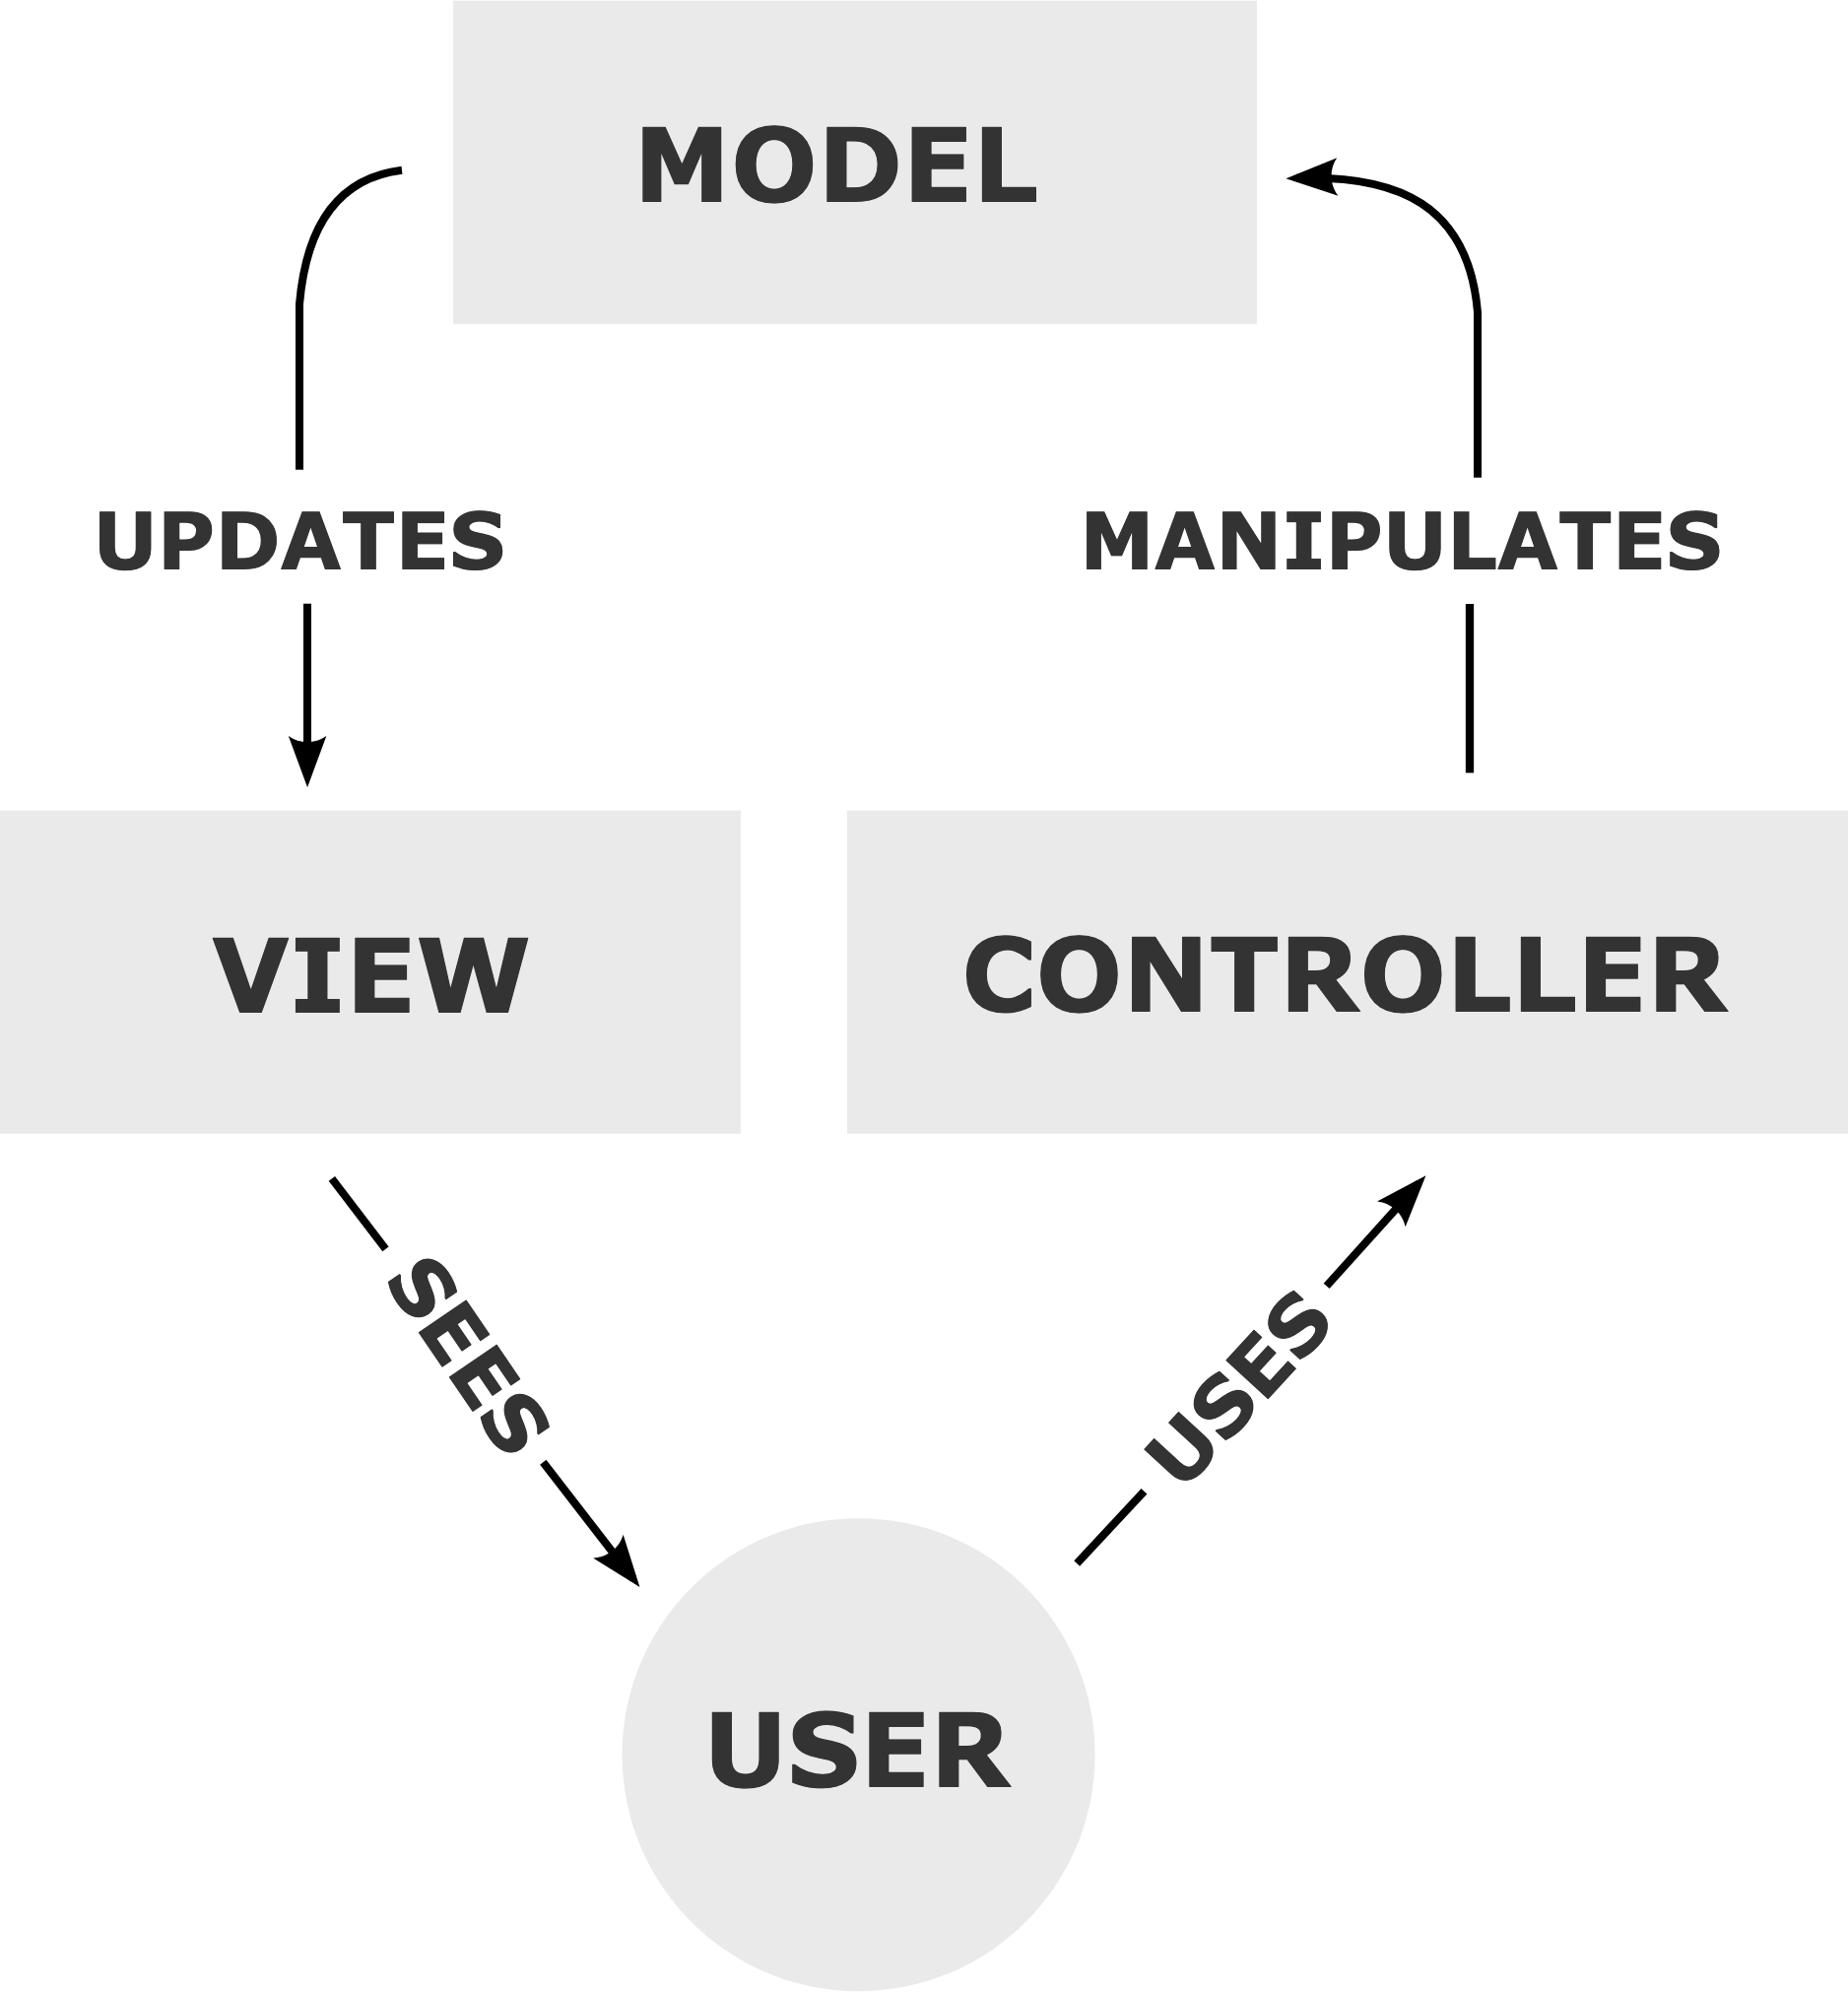
\includegraphics[scale=0.15]{assets/wikipedia_mvc_process}
\end{figure}

\newpage

\subsection{Technische Frameworks}

\subsubsection{Laravel}
Laravel ist ein kostenloses und quelloffenes Framework für die Erstellung moderner PHP Anwendungen.
Es bietet ein umfangreiches Toolset und eine umfangreiche Dokumentation, sowie ein großes Ecosystem weiterer Funktionsbibliotheken und passenden Services.
Laravel bietet eine MVC Architektur, eingebaute Security Features, eine Templating Engine, eine ORM (Object Relational Mapping) Library und vieles mehr.
In den letzten Jahren gewann es schnell an Popularität.
(Vergleiche~\cite{what-is-laravel})

\subsubsection{Laravel Nova}
Um Entwickler dabei zu unterstützen, besonders effizient und einfach, Administrationsinterfaces für Laravel Anwendungen zu entwickeln, wurde ein kostenpflichtiges first-party Framework entwickelt und veröffentlicht (Vergleiche ~\cite{laravel-nova}).
Oftmals haben Laravel Anwendungen eine öffentliche Website, eine API (Programmierschnittstelle) und einen Administrationsbereich für die Verwaltung der Daten (Vergleiche~\cite{laravel-up-and-running}).
Mit Laravel selbst lässt sich sehr gut eine API abdecken, ebenso ist es für öffentliche Websites designt.
Laravel Nova setzt also genau in dem Bereich an, den Entwickler in der Regel individuell aufbauen.

Für Datengetriebene Verwaltungsanwendungen üblich, und auch grundsätzlich durch Laravel vorbereitet, ist eine MVC Architektur.
Durch Nova bleibt allerdings lediglich die Definition des Models, inklusive der Datenbankmigrationen, allerdings fällt die übliche Programmlogik für Controller und View weg.
Stattdessen werden Ressourcen mit Feldern definiert, die je einem Model zugeordnet werden.
Dadurch lässt sich mit deutlich weniger Code, gegenüber einer individuellen Implementierung, die Verwaltung unterschiedlicher Ressourcen aufbauen.
